% sin関数の等間隔補間による比較図

\begin{figure}[H]
  \centering
  \caption{$f(x) = \sin(x)$の等間隔補間（$n=1$次多項式）}
  \label{fig:sin-interp-first}
  \vspace{5pt}
  \begin{minipage}[b]{0.48\linewidth}
    \centering
    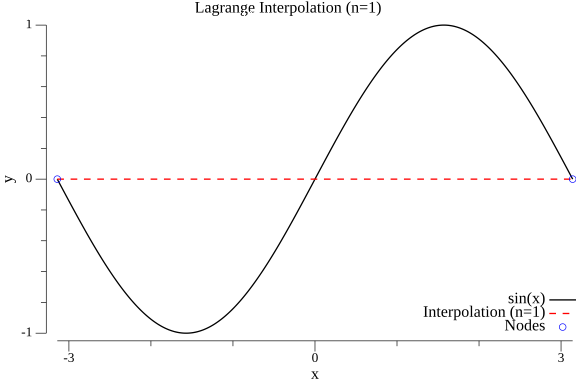
\includegraphics[width=1.0\linewidth]{material/sin/interp/sin_interp_n01.png}
  \end{minipage}
  \hfill
  \begin{minipage}[b]{0.48\linewidth}
    \centering
    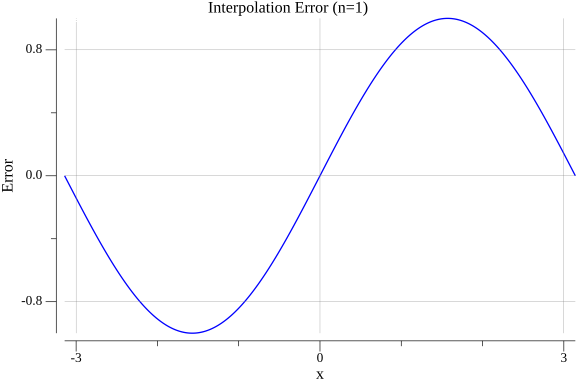
\includegraphics[width=1.0\linewidth]{material/sin/interp/sin_interp_err_n01.png}
  \end{minipage}
\end{figure}

\begin{figure}[H]
  \centering
  \caption{$f(x) = \sin(x)$の等間隔補間（$n=5$次多項式）}
  \label{fig:sin-interp-2}
  \vspace{5pt}
  \begin{minipage}[b]{0.48\linewidth}
    \centering
    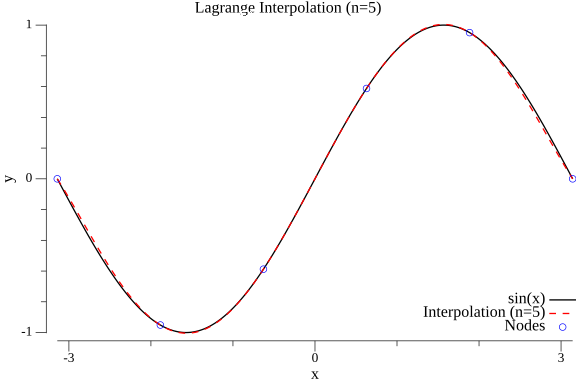
\includegraphics[width=1.0\linewidth]{material/sin/interp/sin_interp_n05.png}
  \end{minipage}
  \hfill
  \begin{minipage}[b]{0.48\linewidth}
    \centering
    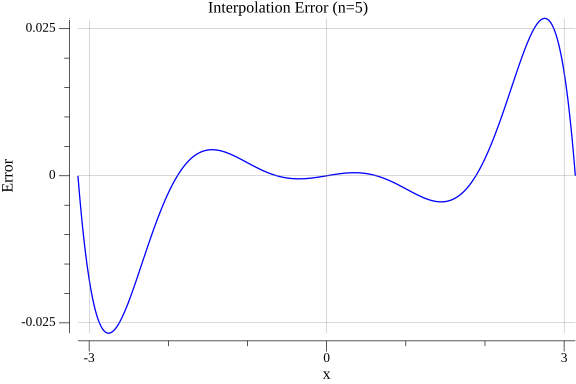
\includegraphics[width=1.0\linewidth]{material/sin/interp/sin_interp_err_n05.png}
  \end{minipage}
\end{figure}

\begin{figure}[H]
  \centering
  \caption{$f(x) = \sin(x)$の等間隔補間（$n=11$次多項式）}
  \label{fig:sin-interp-last}
  \vspace{5pt}
  \begin{minipage}[b]{0.48\linewidth}
    \centering
    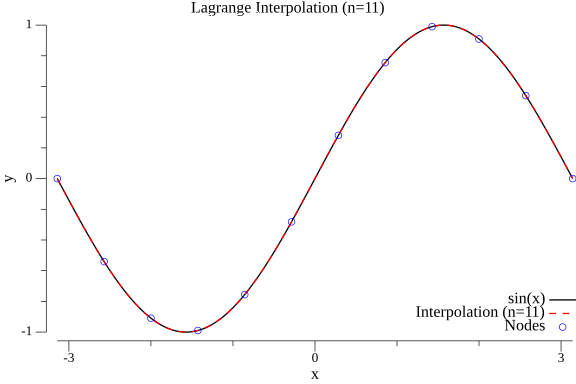
\includegraphics[width=1.0\linewidth]{material/sin/interp/sin_interp_n11.png}
  \end{minipage}
  \hfill
  \begin{minipage}[b]{0.48\linewidth}
    \centering
    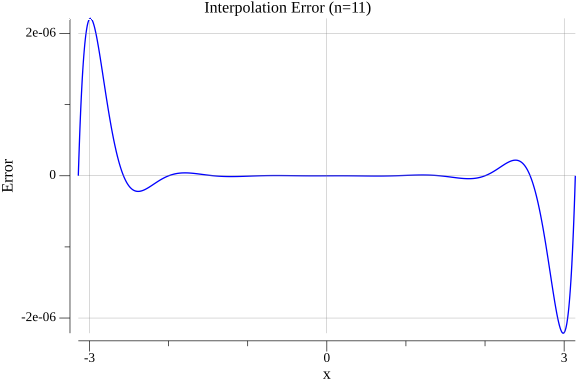
\includegraphics[width=1.0\linewidth]{material/sin/interp/sin_interp_err_n11.png}
  \end{minipage}
\end{figure}

